\documentclass[10pt,a4paper]{article}
\usepackage[T1]{fontenc}
\usepackage{lmodern}
\usepackage[margin=20mm]{geometry}
\usepackage{xurl}
\usepackage{microtype,graphicx,booktabs,tabularx,longtable,enumitem,listings,xcolor,fancyhdr}
\usepackage[colorlinks=true,linkcolor=blue!50!black,urlcolor=blue!50!black]{hyperref}
\definecolor{codebg}{gray}{0.96}
\lstset{basicstyle=\ttfamily\footnotesize,backgroundcolor=\color{codebg},frame=single,rulecolor=\color{black!15},columns=fullflexible,keepspaces=true,breaklines=true,breakatwhitespace=false,showstringspaces=false,upquote=true,xleftmargin=4pt,xrightmargin=4pt}
\setlist{nosep,leftmargin=*}
\setlength{\emergencystretch}{3em}
\setlength{\parindent}{0pt}
\setlength{\parskip}{5pt}
\pagestyle{fancy}\fancyhf{}\fancyhead[L]{\small DAPHNE-M2-004 at CERN}\fancyhead[R]{\small Operator guide, revision 1}\fancyfoot[C]{\thepage}
\setlength{\headheight}{14pt}
\newcommand{\code}[1]{\texttt{\detokenize{#1}}}
\newcommand{\campaign}{\path{/nfs/home/np04daq/vst/daphne-m2-004-offset2250-all32-20261016}}
\newcommand{\field}[1]{\textit{[#1]}}
\title{DAPHNE-M2-004 at CERN\\\large Deployment report and DAPHNE--SSP scan guide}
\author{Prepared for Manuel Arroyave and CERN VST operators}
\date{16 October 2026 \quad | \quad Revision 1}
\begin{document}
\maketitle
\begin{abstract}
DAPHNE-M2-004 replaced DAPHNE-15 in the CERN VST setup. Management access, the 256-sample CAL2 gateware, timing readiness, and acquisition of all 32 firmware channels over two physical data links were exercised. Run 45371 completed five common-VGAIN points with offset DAC 2250. SSP bias and pulse-duration commands were included and read back. The SSP and DAPHNE remain on different timing masters and are not optically coupled in this setup; this result establishes the control and data-taking routine, not a detector gain calibration. This guide records the tested configuration, explains how to repeat it, and supplies a reporting template.
\end{abstract}
\textbf{Recorded final state.} The scan and DAQ run are stopped. All 32 DAPHNE channels are paused; the owned GIB and BOREAS generators are stopped; SSP LED registers are disabled. The DAPHNE endpoint is locked in state 8 with a valid timestamp. These are observations from the completed run, not a live status guarantee for a future operator.

\textbf{Document status.} Operator reference based on campaign evidence; no independent engineering approval is implied. Commands marked as operating instructions are to be run by an authorized operator. Preparing this document did not switch gateware or launch another acquisition.
\newpage
\tableofcontents
\newpage
\section{Deployment report}
\subsection{Installation and network registration}
The installation correspondence records the board as powered with all fibers and serial connected on 16 October 2026. Serial access is through \code{np04-onl-004}. The scan-control host is \code{np04-srv-017}; these hosts have different roles.

Table~\ref{tab:network} records the registered addresses. All five DNS names resolved to the listed IPv4 addresses in the saved CERN-host lookup on 16 October. The MAC associations come from the campaign registration record. Four registered data interfaces do not imply four active physical data links in the loaded firmware.
\begin{table}[ht]
\centering\footnotesize
\begin{tabular}{@{}llll@{}}
\toprule
Interface & Hostname (append \code{.cern.ch}) & Registered MAC & Registered IPv4 \\
\midrule
Management GbE & \code{np04-daphne-m2-004} & \code{00:0A:35:24:05:30} & \code{10.73.137.113} \\
Data d0 & \code{np04-daphne-m2-004-d0} & \code{00:80:55:DE:02:25} & \code{10.73.139.156} \\
Data d1 & \code{np04-daphne-m2-004-d1} & \code{00:80:55:DE:02:26} & \code{10.73.139.159} \\
Data d2 & \code{np04-daphne-m2-004-d2} & \code{00:80:55:DE:02:27} & \code{10.73.139.160} \\
Data d3 & \code{np04-daphne-m2-004-d3} & \code{00:80:55:DE:02:28} & \code{10.73.139.154} \\
\bottomrule
\end{tabular}
\caption{CERN registrations for NP04-DAPHNE-M2-004.}\label{tab:network}
\end{table}

\textbf{Addresses actually used by the loaded data firmware.} The pinned 256-CAL2 sender emits fixed source addresses. The private DAQ configuration was adapted to these values; the CERN reservations were retained.
\begin{center}\small
\begin{tabular}{@{}lll@{}}\toprule
Physical link & Source MAC on the wire & Source IPv4 on the wire \\\midrule
0 & \code{DE:AD:BE:EF:CA:FE} & \code{192.168.0.100} \\
1 & \code{DE:AD:BE:EF:CA:FF} & \code{192.168.0.101} \\\bottomrule
\end{tabular}
\end{center}
Management uses its registered MAC and \code{10.73.137.113/24}, with gateway \code{10.73.137.1}. Optical management was made operational and persisted through \code{daphne-management-optical.service}; persistence across a reboot was not tested.

\subsection{Selectable gateware}
All three profiles have their bitstream and overlay assets installed. Only the 256-CAL2 profile was exercised live in this campaign. Installed availability of the legacy profiles is not a fresh data-taking qualification.
\begin{center}\small
\begin{tabular}{@{}lll@{}}\toprule
Profile & Purpose & Identity build \\\midrule
\code{self-trigger-256-cal2} & 256 samples; guarded CAL2 scans & \code{0x093E0579} \\
\code{self-trigger-1024} & Legacy 1024-sample self-trigger & \code{0x03F17F1B} \\
\code{full-stream} & Legacy full streaming & \code{0x0B24E416} \\\bottomrule
\end{tabular}
\end{center}
The recorded active and boot-default profile is \code{self-trigger-256-cal2}. The additional name \code{self-trigger}, if listed, points to the same installed legacy build as \code{self-trigger-1024}.

\subsection{Completed scan: run 45371}
The final common-gain scan, identified as \code{joint-gain-r4}, set each VGAIN point on all four firmware AFEs before acquisition. Earlier sequential or interrupted attempts remain separate records. Run 45371 also contains earlier activity; use the five receipts in \code{logs/joint-gain-r4.jsonl} to identify this report's selected windows.

At each of five points, all 32 channels supplied 11,626 complete 256-sample frames in a common 2-second readout window. The five selected windows contain 1,860,160 waveforms and 476,200,960 ADC samples. Selected channel timestamps match exactly, with no gaps or duplicates. Over the longer source-active acquisition intervals, each channel's hardware record increment equals 389,061 accepted GIB commands in total; busy/full counts and GIB rejected-command increments were zero. This hardware denominator differs from the smaller set of frames saved in the five selected analysis windows.

\begin{table}[ht]
\centering\small
\begin{tabular}{@{}rrrrr@{}}\toprule
VGAIN code & Pedestal range & Within-frame RMS range & Frames/channel & Clip fractions \\
 & ADC counts & ADC counts & per point & zero / full scale \\\midrule
500 & 4049.57--12647.48 & 2.217--2.488 & 11,626 & 0 / 0 \\
1000 & 6192.90--10299.57 & 1.784--2.089 & 11,626 & 0 / 0 \\
1500 & 7193.72--9205.40 & 1.641--1.934 & 11,626 & 0 / 0 \\
2000 & 7674.53--8670.87 & 1.602--1.897 & 11,626 & 0 / 0 \\
2500 & 7910.10--8415.35 & 1.587--1.932 & 11,626 & 0 / 0 \\
\bottomrule\end{tabular}
\caption{Ranges across all 32 channels; offset DAC 2250. Clip fractions are zero at both ADC rails.}\label{tab:results}
\end{table}

Pedestal is the mean of all raw samples in a channel and point. Within-frame RMS is the square root of the mean per-frame population variance; it excludes changes in each waveform's DC level. Total sample RMS and pedestal drift are also retained in the CSV. All samples were decoded, with no pulse rejection or baseline subtraction. The decoder was cross-checked against \code{fddetdataformats.DAPHNEEthFrame} on frames covering every channel at every point. Larger VGAIN DAC codes must not be described as a measured increase in physical gain: the DAC transfer and detector response were not calibrated here.

\begin{figure}[ht]
\centering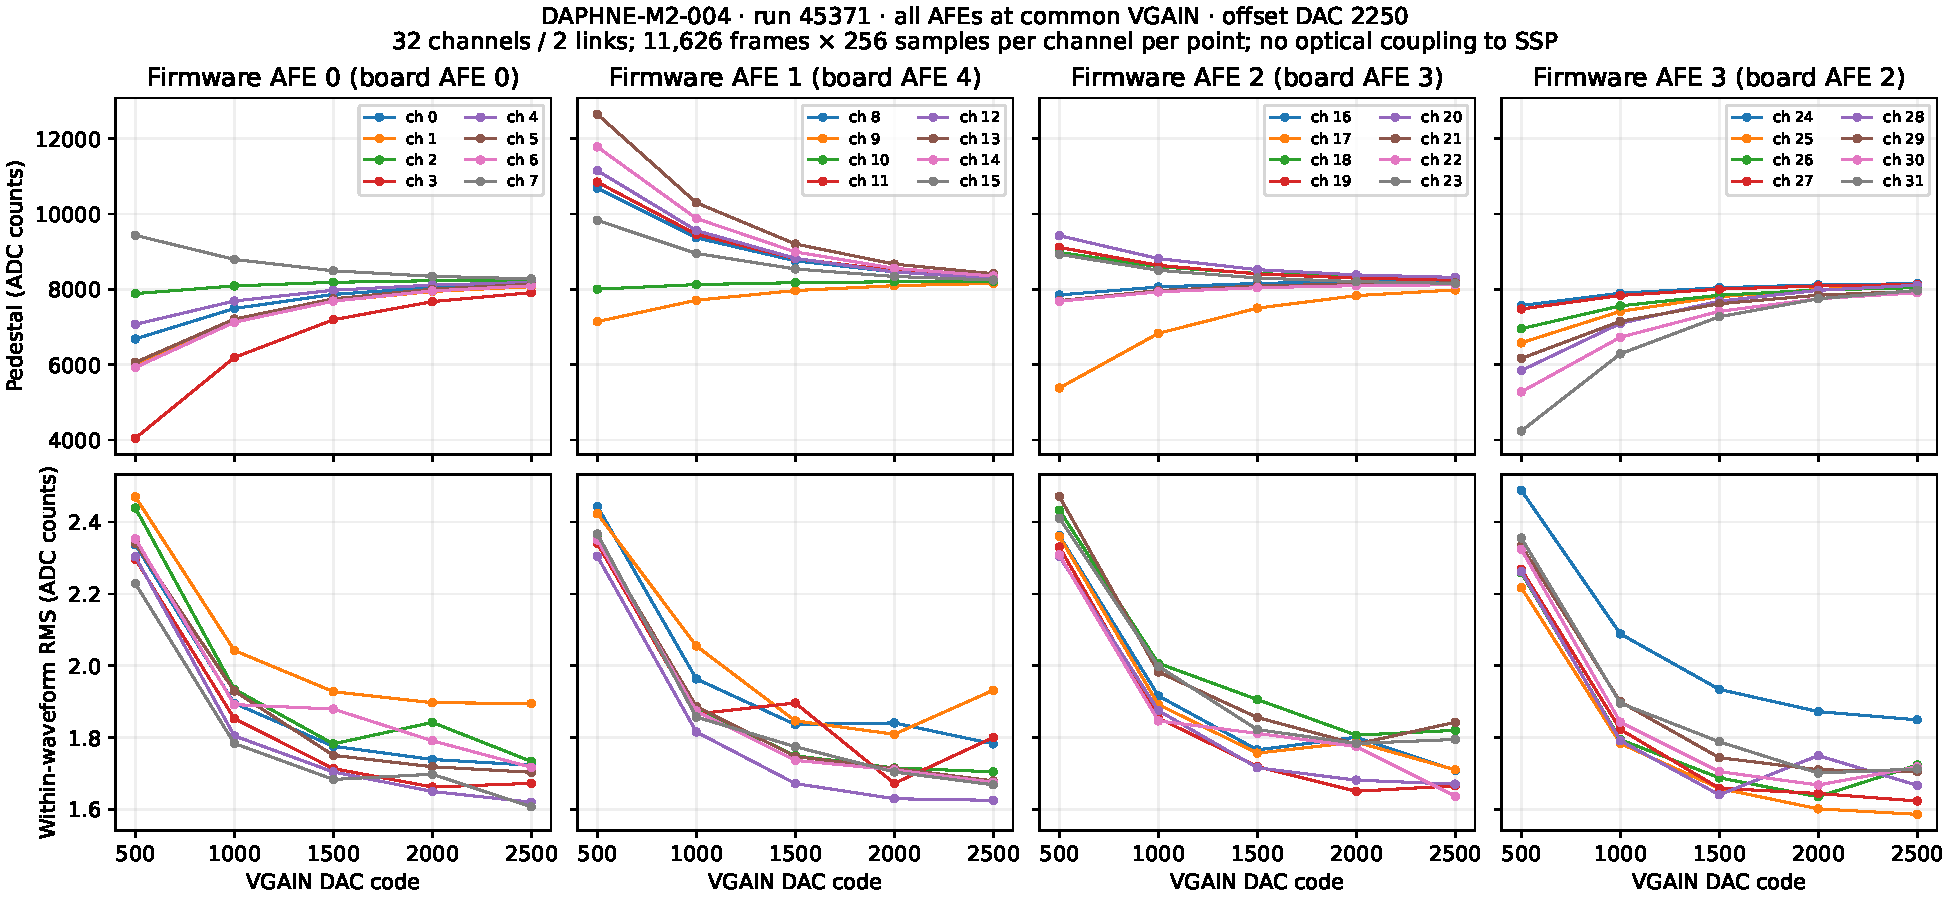
\includegraphics[width=\linewidth]{figures/pedestal-rms.pdf}
\caption{Pedestal and within-frame RMS versus the common VGAIN DAC code. Firmware AFE numbering and physical board AFE numbering are shown separately.}\label{fig:scan}
\end{figure}

SSP bias and pulse-duration register readbacks passed at each point. The SSP command-7 counter increased after starting its BOREAS source. No measured optical output, DAPHNE response to SSP light, or cross-master event synchronization is claimed. No SSP firmware update was performed; SSP activity means LED-control commands and timing-command reception.

\section{Access, host roles, and gateware selection}
\subsection{Access and serial fallback}
Use your authorized CERN access route and credentials. Check tickets on the host from which you connect; do not copy another operator's credential-cache path.
\begin{lstlisting}
klist
# If renewal/login is required, use your own CERN principal:
kinit YOUR_USER@CERN.CH
ssh np04-srv-017
\end{lstlisting}
Scan commands below assume the authorized \code{np04daq} operating account on \code{np04-srv-017}. Board-local commands use:
\begin{lstlisting}
ssh petalinux@np04-daphne-m2-004.cern.ch
\end{lstlisting}
Passwords and private keys are intentionally absent from this handoff.

If management access fails, inspect the serial connection on \code{np04-onl-004}. The observed port is:
\begin{lstlisting}
/dev/serial/by-id/usb-Xilinx_DAPHNE_Mezzanine_004_DAPHNE004-if01-port0
\end{lstlisting}
Use 115200 baud and coordinate ownership before opening a serial terminal. A reachable serial console is a diagnostic path; no reboot is required by this guide.

\subsection{Inspect or switch the FPGA profile}
On the board:
\begin{lstlisting}
sudo /usr/sbin/daphne-gateware list
sudo /usr/sbin/daphne-gateware status
\end{lstlisting}
Stop data taking and stop the scan's timing sources before a switch. Choose one command:
\begin{lstlisting}
# 256-sample CAL2: required for the scan described here
sudo /usr/sbin/daphne-gateware switch self-trigger-256-cal2

# Alternative: legacy 1024-sample self-trigger
sudo /usr/sbin/daphne-gateware switch self-trigger-1024

# Alternative: full streaming
sudo /usr/sbin/daphne-gateware switch full-stream
\end{lstlisting}
The selector stops board runtime services, loads the FPGA app, verifies its identity, and restarts services without rebooting Linux. Re-establish timing and configure DAQ for the selected profile before taking data. Do not apply the CAL2 scan procedure to a legacy profile.

Boot selection is a separate operation:
\begin{lstlisting}
sudo /usr/sbin/daphne-gateware set-default self-trigger-256-cal2
sudo /usr/sbin/daphne-gateware status
\end{lstlisting}
\code{switch} changes the active profile; \code{set-default} changes the next-boot selection. Success requires the expected live identity and healthy runtime services, not just the presence of files.

\section{Configuration of the DAPHNE--SSP exercise}
\subsection{Use the existing CERN campaign}
On \code{np04-srv-017}, as \code{np04daq}:
\begin{lstlisting}
cd /nfs/home/np04daq/vst/daphne-m2-004-offset2250-all32-20261016
source runtime-env.sh
export PYTHONPATH="$PWD:$PDS_PROTOBUF_DIR:$PDS_CHECKOUT/src${PYTHONPATH:+:$PYTHONPATH}"
\end{lstlisting}
The cached environment refers to the installed CERN DAQ/CVMFS software. Use a normal Bash shell; do not enable \code{set -u} while sourcing it. The package supplied with this guide is an archival handoff, not a standalone DAQ installation.

\begin{center}\small
\begin{tabularx}{\linewidth}{@{}lX@{}}\toprule
Item & Tested value \\\midrule
DAPHNE RPC & \code{tcp://np04-daphne-m2-004.cern.ch:40001} \\
Hermes/IPbus & \code{10.73.137.113:50001} \\
DAPHNE endpoint & Address \code{0x16} (22), state 8, clocks locked, timestamp valid \\
DAPHNE source & GIB, generator 1, command 7; requested 6000 Hz \\
Measured source rate & 5812.872 Hz; 10,752 ticks at 62.5 MHz \\
SSP control & \code{10.73.137.61:55002}; endpoint address \code{0x20}, partition 0 \\
SSP source & BOREAS\_TLU\_NP04, generator 1, command 7 \\
DAQ selection & Four source IDs 804--807; 2-second window; 0.5 Hz DAQ triggers \\
DAPHNE settings & All 32 enabled; timing command 7; software trigger disabled; offset DAC 2250 \\
Detector bias & Retain the campaign's zero detector-bias configuration \\
Final scan state & DAPHNE paused; owned timing sources stopped; SSP LED registers disabled \\\bottomrule
\end{tabularx}
\end{center}
Do not conflate the 0.5 Hz DAQ window-request rate with the approximately 5.813 kHz waveform-command rate. The two timing masters are independent. Their timestamps and counters cannot be paired as common events.

\subsection{Channel, link, and source mapping}
\begin{center}\small
\begin{tabular}{@{}rrrrrr@{}}\toprule
Firmware AFE & Board AFE & Firmware channels & Physical link & Wire stream & DAQ source \\\midrule
0 & 0 & 0--7 & 0 & 0 & 804 \\
1 & 4 & 8--15 & 0 & 1 & 805 \\
2 & 3 & 16--23 & 1 & 64 & 806 \\
3 & 2 & 24--31 & 1 & 65 & 807 \\\bottomrule
\end{tabular}
\end{center}
Each physical link carries 16 channels through two 8-channel senders. Physical board AFE 1 is not represented in these 32 firmware channels. The runtime adapter translates firmware channel numbers to physical board channels.

The firmware's wire stream IDs are \code{0,1,64,65}. The campaign's \code{acquisition_wire_ids.py} validates this exact mapping. A generic decoder that expects \code{0,1,2,3} will reject the second link. Keep the corrected DAQ GeoIDs and this acquisition adapter together. The current sender's legacy UDP counters may remain zero; use waveform receipts and hardware record/busy/full counters for these acceptance checks.

\subsection{SSP recipe and scan transaction}
The recipe exercised SSP channels 0--2 (mask \code{7 = 0x007}), with 12 controller channels configured in single-pulse mode:
\begin{lstlisting}[language=Python]
plan['illumination']['settings'] = {
    'led_bias_270nm': 4095,
    'led_bias_367nm': 0,
    'led_width_ticks': 8,
    'led_second_width_ticks': 1,
    'led_double_pulse_delay_ticks': 4000,
    'led_channel_mask': 7,
    'led_burst_count': 1,
}
\end{lstlisting}
The values are native driver codes and controller ticks. Despite the driver's internal bias-field naming, do not present \code{4095} as a percentage or convert widths to nanoseconds without establishing the controller clock. The second-pulse and delay fields are recorded while pulse mode is single; they do not establish that a double pulse was emitted. SSP LED bias is distinct from DAPHNE detector bias.

For each VGAIN point the runner:
\begin{enumerate}
\item Pauses and drains all four firmware AFEs. It programs all offsets and the common VGAIN while acquisition remains paused.
\item Configures SSP bias and timing fields, verifies all 12 register pairs, and starts the owned BOREAS generator. It requires an increasing SSP command-7 counter.
\item Arms CAL2 for all 32 channels and releases their pause mask together. It snapshots DAPHNE counters and starts the owned GIB generator.
\item Selects a complete, stable, closed HDF5 window from all four sources. It checks headers, timestamps, coverage, duplicate events, and fragment status.
\item Stops GIB, checks hardware counters against accepted commands, pauses DAPHNE, and advances to the next common gain.
\end{enumerate}
SSP commands continue on BOREAS between DAPHNE acquisition windows until reconfigured or stopped. Cleanup stops both owned sources and disables SSP LED registers. A readback confirms controller state; it is not an optical measurement.

\section{Repeat the common-gain scan}
\subsection{Check readiness and DAQ state}
Before starting, confirm the active gateware is 256-CAL2, both data links are ready, DAPHNE is in state 8 with valid timestamps, and SSP is in state 8 with its ready bit set. Ensure the campaign's timing generators are available and no other scan owns them. The runner reserves its masters and checks GIB readiness; SSP checks happen before its first configuration.

Use the existing dedicated DAQ session:
\begin{lstlisting}
tmux attach -t pds-vst-m2-004-offset2250-all32
\end{lstlisting}
In its DAQ window, the recorded idle state is \code{configured} with no applications in error. The initialized session already contains the corrected four-source configuration. If the session is missing, or gateware/timing/configuration has changed, have the DAQ owner initialize the campaign before continuing. Do not rerun historical preparation or recovery scripts blindly: some rewrite configuration or manipulate runtime state.

\subsection{Create fresh output names before acquisition}
Run this in a second operator terminal in the campaign directory. Choose a new tag; the example \code{r5} must be unused.
\begin{lstlisting}
python3 - <<'PY_NEW'
from pathlib import Path
r = Path('.')
tag = 'r5'  # choose a fresh tag
paths = [r / f'run-joint-gain-{tag}.py',
         r / f'plans/joint-gain-{tag}.json',
         r / f'logs/joint-gain-{tag}.jsonl',
         r / f'data/calibration/joint-gain-{tag}']
if any(p.exists() for p in paths):
    raise SystemExit('Tag already used; choose another tag')
text = (r / 'run-joint-gain-r4.py').read_text()
with paths[0].open('x') as output:
    output.write(text.replace('r4', tag))
print('Created', paths[0])
PY_NEW
\end{lstlisting}
The preparation checks that the script and all three output paths are fresh. If any exists, select a new tag and start from the original runner. The runner opens its plan and journal exclusively and does not overwrite a prior dataset. Keep all paths for a scan under the same new tag.

Edit \code{run-joint-gain-r5.py} before starting. The \code{plan} dictionary contains the common gain list. The tested list is \code{[500,1000,1500,2000,2500]}. All firmware AFEs \code{[0,1,2,3]} and channels \code{0..31} remain selected. Add an explicit SSP settings block, as shown above, immediately after the \code{plan} dictionary and before the line that writes the plan JSON. This overrides the settings otherwise inherited from \code{plans/offset2250-afe0-r3.json}, without modifying that historical plan.

\textbf{Current interface limitation.} This campaign runner embeds its configuration in Python; \path{plans/joint-gain-r4.json} is the saved record, not a generic input accepted by the runner. Merely editing a saved JSON will not drive a new scan. Offset 2250 and the acquisition window also appear in hardware-write/receipt code. Retain those tested values for a repeat; changing them requires consistent code and DAQ configuration review. The generic single-AFE \code{pds-calibrate} interface is not a substitute for this simultaneous four-AFE runner.

\subsection{Start one DAQ run and launch the scan}
At the dedicated DAQ prompt:
\begin{lstlisting}
start-run --run-type TEST
\end{lstlisting}
Wait for success and record the new run number. In the new runner, replace the \code{run_number} value \code{45371} with the actual new run number before launching. It is report metadata, not a command to select the DAQ run. The runner checks fresh HDF5 timestamps but does not enforce the run number in filenames, so the operator must confirm the active run and selected receipt filenames agree.

From the second terminal, after sourcing the environment described above:
\begin{lstlisting}
set -o pipefail
"$PDS_VENV/bin/python" -u run-joint-gain-r5.py \
    2>&1 | tee run-joint-gain-r5.console.log
\end{lstlisting}
Stay connected until cleanup completes, or run this command in a dedicated operator-owned terminal multiplexer window. The timing workers have bounded lifetimes, but that is not a replacement for checking cleanup.

Expected journal events are \code{point_configured}, \code{point_started}, and \code{point_complete} for every gain, followed by \code{all_points_complete} and \code{final_cleanup}. Each point must show 32 channels, identical event timestamps across those channels, no missing/duplicate waveforms, zero busy/full increments, and zero rejected GIB commands. Expect roughly 11,626 waveforms per channel in a 2-second window; the exact integer depends on the clock phase and recorded source period.

After cleanup, issue at the DAQ prompt:
\begin{lstlisting}
stop-run
\end{lstlisting}
Confirm all applications return to configured/idle with no errors. Record endpoint readiness, final pause mask \code{0xffffffff}, SSP LED registers disabled, and the source-stop acknowledgements.

\subsection{Interrupts and failures}
Interrupt the foreground runner with Ctrl-C, or send SIGTERM only to the identified scan process. The main runner catches these through its cleanup path. Avoid a forced kill if cleanup can run. Confirm the \code{final_cleanup} journal event; an attempted cleanup is not proof that every action succeeded.

If endpoint readiness, register acknowledgement, counter equality, or data integrity fails, preserve the failed journal and do not describe the point as a calibration result. Stop the run, verify that owned timing sources are stopped and SSP LEDs are disabled, and involve the corresponding timing/DAQ owner before retrying. Do not disable strict data checks or change ownership of another user's timing generator.

\section{Decode, assess, and write the report}
\subsection{Keep raw data, receipts, and checksums}
A successful control loop is one part of acceptance. Decode every selected channel and point, verify each binary's receipt SHA-256, and check pedestal, total RMS, within-frame RMS, waveform-mean drift, and fractions at ADC values 0 and 16383. Cross-check the ADC unpacking against the official frame decoder. Changing pedestal and noise with VGAIN is expected in this electronics exercise; neither quantity alone establishes detector gain.

The archived \path{support/decode-joint-gain-r4.py} contains the run-45371 analysis procedure and original CERN paths. Its output directory already exists in the reference campaign, so an unchanged rerun deliberately fails rather than overwriting evidence. It deliberately uses the r4 journal and a fresh analysis directory. For another run, make a separate decoder copy, update its journal/analysis paths and run metadata, and update its expected gain list and point count if those changed. Do not run it unchanged against a new run or overwrite the original analysis. Verify the configured common gain in each journal against each dataset receipt.

For the reference scan, retain these files relative to the CERN campaign:
\begin{lstlisting}
plans/joint-gain-r4.json
logs/joint-gain-r4.jsonl
data/calibration/joint-gain-r4/step-000.bin  # through step-004.bin
data/calibration/joint-gain-r4/step-000.json # through step-004.json
analysis-joint-gain-r4/analysis.json
analysis-joint-gain-r4/channel-statistics.csv
analysis-joint-gain-r4/evidence.json
\end{lstlisting}
Receipt fields identify the source HDF5 file, record ID, common readout window, counts, and payload hash. Preserve the original HDF5 files too. The handoff archive includes the report, numeric analysis, journals, hashes, and support code; the large raw HDF5 and waveform binaries remain on CERN storage.

\subsection{Minimum contents of a future scan report}
Use \code{report-template.tex} as an editable companion. Fill in measured values rather than copying the reference result:
\begin{enumerate}
\item Identify the operator, date/time zone, board, physical connections, control host, campaign path, scan tag, DAQ run number, and purpose.
\item Record active gateware identity, source revision/dirty state, bitstream/overlay/server hashes, environment, and any changes since this reference.
\item State both physical and logical topology: two links, four wire streams, source IDs, firmware-to-board AFE mapping, and channel selection.
\item List offset, gain points, SSP mode/mask/bias/width/delay/burst settings, native units, and detector-bias state separately.
\item Record both timing masters, source period/rate, endpoint states, and whether optical coupling or a shared clock exists.
\item Report acceptance using explicit observation points and denominators: selected window waveforms per channel versus full hardware-counter intervals. Include losses, rejections, clipping, and pedestal/RMS plots.
\item State final cleanup, remaining problems, and what was not demonstrated. Link immutable receipts, raw files, scripts, configuration, and checksums.
\end{enumerate}

\subsection{Suggested short report for this installation}
\begin{quote}
NP04-DAPHNE-M2-004 is reachable through its registered management address, 10.73.137.113. The 256-sample CAL2, legacy 1024-sample self-trigger, and full-stream profiles are installed and selectable with the board's daphne-gateware utility. The 256-CAL2 profile is the recorded active and boot-default selection.

Run 45371 completed a common-VGAIN scan at codes 500, 1000, 1500, 2000, and 2500, with offset DAC 2250 on all 32 firmware channels over two physical data links. Each selected point contains 11,626 aligned waveforms per channel. Decoding and integrity checks passed, with no observed ADC rail clipping; hardware record counters matched accepted GIB commands with zero busy/full or rejected-command increments over the measured intervals.

SSP LED bias and duration controls were exercised with register readback and command-counter response. The SSP remains on BOREAS\_TLU\_NP04 while DAPHNE uses GIB, and the SSP is not optically coupled to DAPHNE-004. Optical detector response and shared-master synchronization remain to be tested when both systems are installed together. The run ended with DAPHNE paused, owned timing sources stopped, and SSP LEDs disabled.
\end{quote}

\appendix
\section{Timing compatibility note for the pinned 256-CAL2 build}
During this campaign the DAPHNE endpoint remained in deskew-wait state 6 after the standard GIB delay/resync sequence. The pinned endpoint clears \code{ddone} on command 4. After the normal sequence had been completed, a targeted endpoint command 3 restored state 8 and a valid timestamp:
\begin{lstlisting}[language=Python]
# Historical targeted correction, not an unconditional initialization step.
# Device d is GIB from /nfs/sw/dunedaq/timing/connections.xml.
packet = [0x16, 0, 0xab, 0xf0, 0x81, 0x103]
d.getNode('master').transmit_async_packet(packet, -1)
\end{lstlisting}
This is recorded to help a timing owner reproduce the diagnosis. It is not a master reset or an instruction to repeat writes on an already ready endpoint. Coordinate access, verify the pinned build and endpoint address, stop periodic sources, and confirm the prior standard sequence before applying any recovery. The exact executed procedure is retained in the original deployment campaign as \code{operator-deskew-completion.sh} and \code{logs/deskew-completion.json}.

\section{Provenance and handoff files}
The deployment record and the final scan record serve different purposes. The initial deployment result describes the earlier limited run 45368; it must not be used as the final all-32-channel result. This guide's quantitative findings use run 45371, \code{joint-gain-r4}.

\begin{description}[style=nextline]
\item[Original deployment campaign]
\path{/nfs/home/np04daq/vst/daphne-m2-004-20261016}
\item[Final common-gain campaign]
\campaign
\item[Runtime PDS checkout]
\path{/nfs/home/np04daq/calib/control/PDS}; commit \code{82fa12eeefef2d480fc23e869ad2c9c2bc54017b}, with local documentation/tool changes recorded in the evidence manifest.
\item[Official frame decoder]
\code{fddetdataformats} commit \code{75451f42c049bf51132493075d61a1c884592425}; clean source state at analysis.
\item[FPGA source]
\code{93e05798ac1680b254760146974e95891863d2eb}; live identity \code{0x093e0579}.
\item[Server]
\path{/opt/daphne-server/cal2-vst-frame-monitor-20261008/bin/daphneServer}; source base \code{258cc46} plus the recorded local CAL2 frame-monitor fix. A source base commit alone does not reproduce this dirty snapshot.
\end{description}
The loaded OS was PetaLinux; an exact OS image digest was not established in this handoff. Keep that qualification separate from the verified FPGA/overlay/server artifacts.

\small
\begin{lstlisting}
256-CAL2 bitstream SHA-256:
3e91c1dfa956776b18f6dc90d58179d5552b70ae99639fd36b64809fed68ab8a
Board-compatible overlay SHA-256:
828e42e8e467d0208b895fa63e3274a5bfc3446c0668c5984d00301087273e21
Server binary SHA-256:
6b786fa74f6c73e8f23af957bd5f55746b9a5774bc7913c0a37eef439505f82c
Joint gain runner SHA-256:
db7eb53c32229acb092b0fd65ccb4fbc16dc5e46e95f3f2aade30bed2910b808
Wire-ID acquisition adapter SHA-256:
43f31239c5fee7d44dd90299ab40b37ac0827aa64b7aec64a3f2e49ab18c4355
\end{lstlisting}
\normalsize
In the portable handoff, \code{evidence/evidence.json} records the complete analysis hashes, source states, original HDF5 hashes, acceptance results, and limitations. \code{evidence/analysis.json} holds the full channel statistics and receipts; \code{evidence/channel-statistics.csv} is convenient for independent plotting. The \code{support/} directory contains the archived scan, acquisition, and SSP-control code plus its original cached environment and base plan.

Build this document with Tectonic, or use a LaTeX distribution that supplies the listed packages:
\begin{lstlisting}
tectonic daphne-m2-004-guide.tex
tectonic report-template.tex
# Alternative: run pdflatex twice on the guide for its contents/references.
\end{lstlisting}
The guide is a reproducible record and operator reference. Hardware use still requires the installed CERN environment, authorized accounts, correct cabling, and ownership of the indicated DAQ/timing resources.
\end{document}
